
\subsection*{The Story of Your Life}

%%%Insert this to get the typewriter font so it looks like a real movie script
{\ttfamily
\fontdimen2\font=0.4em
\fontdimen3\font=0.2em
\fontdimen4\font=0.1em
\fontdimen7\font=0.1em
\hyphenchar\font=`\-


%%%%put a hypertarget around the opening bit of text
\hypertarget{vectors_in_space_n_vectors_hint}{This video talks about the} weird notion of
a ``length-squared'' for a vector $v=(x,t)$ given by $||v||^2=x^2-t^2$ used in Einstein's theory of relativity.
The idea is to plot the story of your life on a plane with coordinates $(x,t)$. The coordinate $x$ encodes
{\it where} an event happened (for real life situations, we must replace $x\to (x,y,z)\in {\mathbb R}^3$). 
The coordinate $t$ says {\it when} events happened. Therefore you can plot your life history as a worldline
as shown:
\begin{center}
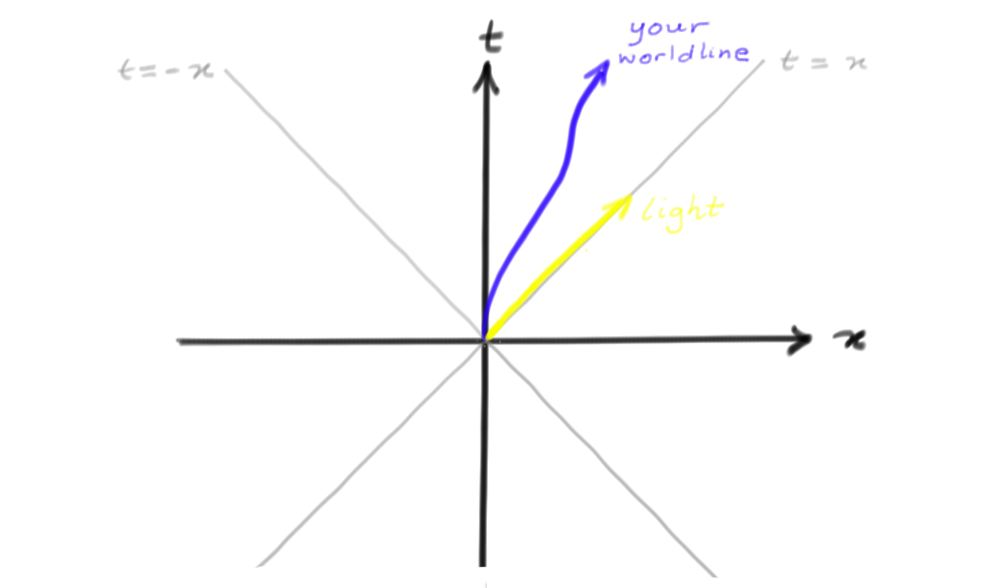
\includegraphics[scale=.2]{worldline.jpg}
\end{center}
Each point on the worldline  corresponds to a place and time of an event in your life. The slope of
the worldline has to do with your speed. Or to be precise, the inverse slope is your velocity. 
Einstein realized that the maximum speed possible was that of light, often called $c$. In the diagram above
$c=1$ and corresponds to the lines $x=\pm t\Rightarrow x^2-t^2=0$. This should get you started in your search for vectors
with zero length.




%%%%don't forget to close the bracket so the stuff after your file doesn't look like a movie!
}

%\newpage
